\documentclass{beamer}
\mode<presentation>
\usepackage{amsmath,amssymb,mathtools}
\usepackage{textcomp}
\usepackage{gensymb}
\usepackage{adjustbox}
\usepackage{subcaption}
\usepackage{enumitem}
\usepackage{multicol}
\usepackage{listings}
\usepackage{url}
\usepackage{graphicx} % <-- needed for images
\def\UrlBreaks{\do\/\do-}

\usetheme{Boadilla}
\usecolortheme{lily}
\setbeamertemplate{footline}{
  \leavevmode%
  \hbox{%
  \begin{beamercolorbox}[wd=\paperwidth,ht=2ex,dp=1ex,right]{author in head/foot}%
    \insertframenumber{} / \inserttotalframenumber\hspace*{2ex}
  \end{beamercolorbox}}%
  \vskip0pt%
}
\setbeamertemplate{navigation symbols}{}

\lstset{
  frame=single,
  breaklines=true,
  columns=fullflexible,
  basicstyle=\ttfamily\tiny   % tiny font so code fits
}

\numberwithin{equation}{section}

% ---- your macros ----
\providecommand{\nCr}[2]{\,^{#1}C_{#2}}
\providecommand{\nPr}[2]{\,^{#1}P_{#2}}
\providecommand{\mbf}{\mathbf}
\providecommand{\pr}[1]{\ensuremath{\Pr\left(#1\right)}}
\providecommand{\qfunc}[1]{\ensuremath{Q\left(#1\right)}}
\providecommand{\sbrak}[1]{\ensuremath{{}\left[#1\right]}}
\providecommand{\lsbrak}[1]{\ensuremath{{}\left[#1\right.}}
\providecommand{\rsbrak}[1]{\ensuremath{\left.#1\right]}}
\providecommand{\brak}[1]{\ensuremath{\left(#1\right)}}
\providecommand{\lbrak}[1]{\ensuremath{\left(#1\right.}}
\providecommand{\rbrak}[1]{\ensuremath{\left.#1\right)}}
\providecommand{\cbrak}[1]{\ensuremath{\left\{#1\right\}}}
\providecommand{\lcbrak}[1]{\ensuremath{\left\{#1\right.}}
\providecommand{\rcbrak}[1]{\ensuremath{\left.#1\right\}}}
\theoremstyle{remark}
\newtheorem{rem}{Remark}
\newcommand{\sgn}{\mathop{\mathrm{sgn}}}
\providecommand{\abs}[1]{\left\vert#1\right\vert}
\providecommand{\res}[1]{\Res\displaylimits_{#1}}
\providecommand{\norm}[1]{\lVert#1\rVert}
\providecommand{\mtx}[1]{\mathbf{#1}}
\providecommand{\mean}[1]{E\left[ #1 \right]}
\providecommand{\fourier}{\overset{\mathcal{F}}{ \rightleftharpoons}}
\providecommand{\system}{\overset{\mathcal{H}}{ \longleftrightarrow}}
\providecommand{\dec}[2]{\ensuremath{\overset{#1}{\underset{#2}{\gtrless}}}}
\newcommand{\myvec}[1]{\ensuremath{\begin{pmatrix}#1\end{pmatrix}}}
\newcommand{\mydet}[1]{\ensuremath{\begin{vmatrix}#1\end{vmatrix}}}

\newenvironment{amatrix}[1]{%
  \left(\begin{array}{@{}*{#1}{c}|*{#1}{c}@{}}
}{%
  \end{array}\right)
}

\newcommand{\myaugvec}[2]{\ensuremath{\begin{amatrix}{#1}#2\end{amatrix}}}
\let\vec\mathbf
% ---------------------

\title{Matgeo Presentation - Problem 12.589}
\author{ee25btech11056 - Suraj.N}

\begin{document}

\begin{frame}
  \titlepage
\end{frame}

\begin{frame}{Problem Statement}

Solve the system of equations and find the condition for which the system has \textbf{no solution}:

\begin{align*}
x+y+z &= 6 \\
x+4y+6z &= 20 \\
x+4y+\lambda z &= \mu
\end{align*}

\end{frame}

\begin{frame}{Data}

\begin{table}[h!]
  \centering
  \begin{tabular}{|c|c|}
\hline
\textbf{Name} & \textbf{Value} \\ \hline
$\vec{A}$ & $\myvec{2 & 1 \\0 & 3}$ \\ \hline
\end{tabular}

  \caption*{Table : Equations}
  \label{12.589}
\end{table}

\end{frame}

\begin{frame}{Solution}

The system of equations in matrix form is :
\begin{align}
\myvec{1 & 1 & 1\\1 & 4 & 6\\1 & 4 & \lambda}\myvec{x\\y\\z} &= \myvec{6\\20\\\mu}
\end{align}

Forming the augmented matrix,
\begin{align}
\myaugvec{3}{1 & 1 & 1 & 6\\1 & 4 & 6 & 20\\1 & 4 & \lambda & \mu}
\end{align}

Using Gaussian elimination,
\begin{align}
\myaugvec{3}{1 & 1 & 1 & 6\\1 & 4 & 6 & 20\\1 & 4 & \lambda & \mu}
\xleftrightarrow[\;R_2 \to R_2 - R_1\;]{\;R_3 \to R_3 - R_1}
\myaugvec{3}{1 & 1 & 1 & 6\\0 & 3 & 5 & 14\\0 & 3 & \lambda-1 & \mu-6}
\end{align}

\begin{align}
\myaugvec{3}{1 & 1 & 1 & 6\\0 & 3 & 5 & 14\\0 & 3 & \lambda-1 & \mu-6}
\xleftrightarrow{R_3 \to R_3 - R_2}
\myaugvec{3}{1 & 1 & 1 & 6\\0 & 3 & 5 & 14\\0 & 0 & \lambda-6 & \mu-20}
\end{align}

\end{frame}

\begin{frame}{Solution}

From back substitution we get:
\begin{align}
(\lambda-6)z &= \mu-20
\end{align}

For the system to have \textbf{no solution}, we must have
\begin{align}
  \lambda &= 6 & \mu \neq 20
\end{align}

So, we get zero equal to a non-zero value which is not possible .\\
Therefore the system of equations has \textbf{no solution}.

\textbf{Final Answer :} The system has no solution when $\lambda=6$ and $\mu \neq 20$.

\end{frame}

\begin{frame}{Plot}

\begin{figure}[h!]
  \centering
  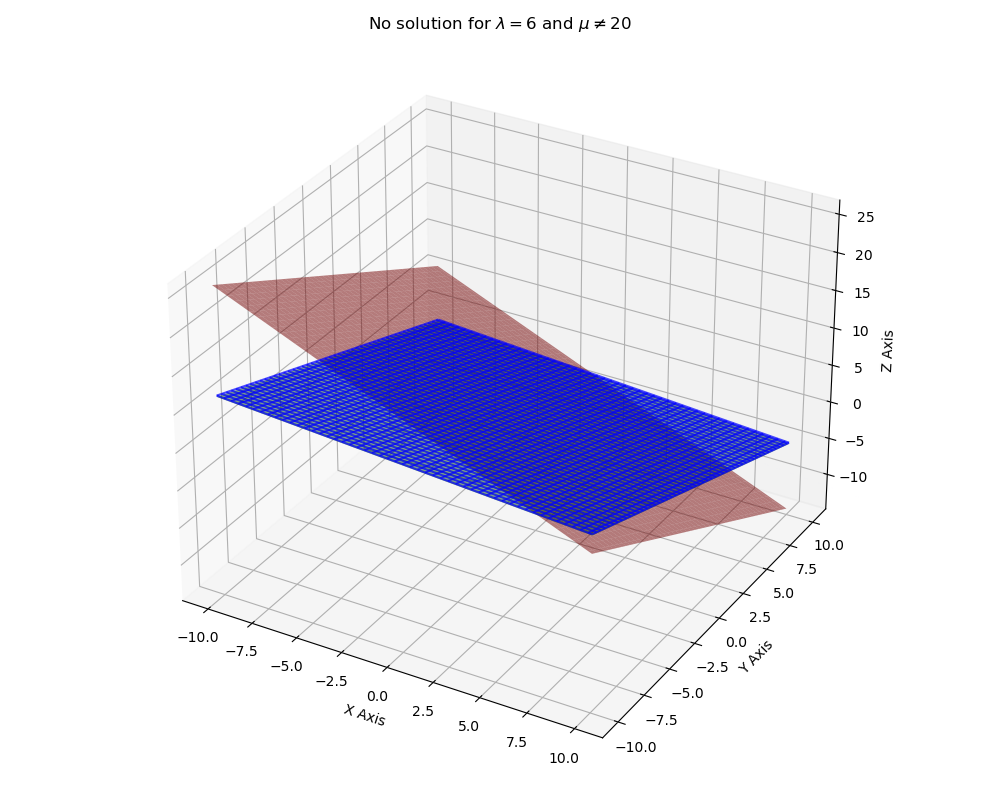
\includegraphics[width=0.8\columnwidth]{figs/planes.png} 
   \caption*{Fig : Planes}
  \label{Fig1}
\end{figure}

\end{frame}


\end{document}

